\documentclass{article}
\usepackage{amsmath, amssymb, tikz}

\begin{document}

\textbf{Action Principle}

Recall Fermat's Principle: Light travels along the shortest path between 2 points.

Precisely: \quad \textit{length of a curve} \quad $L = \int ds \sqrt{ \left( \frac{dx}{ds} \right)^2 + \left( \frac{dy}{ds} \right)^2 }$ \quad will be minimized for the trajectory of light.

\begin{itemize}
    \item Every mechanical system obeys a minimization principle of this sort.
\end{itemize}

$\rightarrow$ Consider the set of all possible paths $q_i(t)$ that a system could take through configuration space.

Define the action if a path $q_i(t)$: \quad $S[q_i(t)] = \int_{t_i}^{t_f} L(q_i, \dot{q}_i, t) \quad (q_i, \dot{q}_i \Rightarrow \text{the path we choose})$

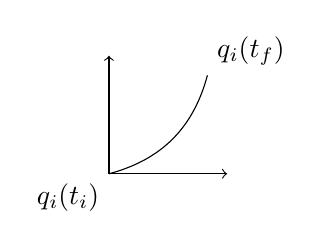
\begin{tikzpicture}[scale=0.5, baseline=(current bounding box.center)]
    \draw[->] (0,0) -- (3,0);
    \draw[->] (0,0) -- (0,3);
    \draw (0,0) node[below left] {$q_i(t_i)$} to[bend right] (2.5,2.5) node[above right] {$q_i(t_f)$};
\end{tikzpicture}
\quad (configuration space / space of all $q_i$'s)

\quad depends on $q_i(t)$ (function of a function)

The path through configuration space that a mechanical system takes "minimize" $S[q_i(t)]$ (minimize implies "local extremum")

This is called the least action principle or Hamilton's principle.

$S[q_i(t)]$ is a function of a function

\textit{"Functionals"}: use $[ \ ]$ rather than $( \ )$ to denote dependence.

\textbf{Calculus of variations}: We have used in single (or multi) variable calculus to minimizing a function of 1 (or $n$) variables.

We need to minimize a \textit{functional} $\Rightarrow$ a function of an $\infty$ \# of variables.

$S[q(t)]$ \quad $\xrightarrow{\text{infinit set of variables}}$

\end{document}